\documentclass[a4paper,11pt]{article}
\usepackage{geometry}
 \geometry{
 a4paper,
 total={170mm,257mm},
 left=20mm,
 top=20mm,
 }



 \usepackage{amsmath}
 \usepackage{siunitx}
 \usepackage{multirow}
\usepackage{colortbl}
 \usepackage{hhline}

 \usepackage{lipsum}  %%% Lorem ipsum

\setlength{\headheight}{30.0pt}
\setlength{\footskip}{20pt}


\usepackage{hyperref}
\hypersetup{
    colorlinks=True,
    linkcolor={blue!20!black},
    filecolor=magenta,      
    urlcolor=cyan,
}



 \usepackage[export]{adjustbox}
\usepackage[english]{babel}
\usepackage[utf8]{inputenc}
\usepackage{fancyhdr}
\usepackage{multicol}

\pagestyle{fancy}
\fancyhf{}
\rhead{\textit{Pul074BEX004}}
\lhead{\textit{Amrit Prasad Phuyal}}
\rfoot{\thepage}


\usepackage{mathpazo} % Palatino font
\usepackage{graphicx}
\usepackage{float}
\usepackage{xcolor}
\usepackage{color}

%%%% Anser environment use %%%% Anser environment use %%%% Anser environment use \input{./AnsENV.tex}
%% use \begin{A... {**** argument***}
\RequirePackage{scrextend}

\newenvironment{A}[1]{\textit{Answer:}{\begin{addmargin}[2em]{2em}{#1}\end{addmargin} 
  }}

% just leave some space   
%% use \begin{A... {**** argument***}
\RequirePackage{scrextend}

\newenvironment{A}[1]{\textit{Answer:}{\begin{addmargin}[2em]{2em}{#1}\end{addmargin} 
  }}

% just leave some space   
%% use \begin{A... {**** argument***}
\RequirePackage{scrextend}

\newenvironment{A}[1]{\textit{Answer:}{\begin{addmargin}[2em]{2em}{#1}\end{addmargin} 
  }}

% just leave some space    %% Answer environment 

%%% Question Environment%%%  use 
%%% Question Environment%%%  use 
%%% Question Environment%%%  use \input{./QueENV.tex}   to include
%% Use \begin{Q}....\end{Q}

\newcounter{QC}
\setcounter{QC}{1}
\newenvironment{Q}[1]{
    \section{Question -\arabic{QC}} \stepcounter{QC}{\large\textbf{#1}}
}

%%% Question Environment%%%

   to include
%% Use \begin{Q}....\end{Q}

\newcounter{QC}
\setcounter{QC}{1}
\newenvironment{Q}[1]{
    \section{Question -\arabic{QC}} \stepcounter{QC}{\large\textbf{#1}}
}

%%% Question Environment%%%

   to include
%% Use \begin{Q}....\end{Q}

\newcounter{QC}
\setcounter{QC}{1}
\newenvironment{Q}[1]{
    \section{Question -\arabic{QC}} \stepcounter{QC}{\large\textbf{#1}}
}

%%% Question Environment%%%

 %% Question Environment 
%%%%%% include  Titles.%%%% use \input{./CP}%%%
%%%use """"""""    \CP{}{}{}{}   """" %%%% and 4 argument to craete Title page 
%%%%%%%%%%%%%%%%%%%%%%%%%%%%%%%%%%%%%%%%%%%%%%%%%%%%%%%%%%%%%%%%%
%%%argument number
%% 1=major header ## Course name 
%% 2=minor4 heading ## lab/assignmet no
%% 3=Title  ## Assignment or Lab title
%% 4=submitted to::## input receiver Name"
%%%%%%%%%%%%%%%%%%%%%%%%%%%%%%%%%%%%%%%%%%%%%%%%%%%%%%%%%%%%%%%%%


\usepackage{mathpazo} % Palatino font
\usepackage{graphicx}
\usepackage{float}

%%% format and command for lab ans c and assembly

\newcommand{\HRule}{\rule{\linewidth}{0.4mm}} % Defines a new command for horizontal lines, change thickness here



%----------------------------------------------------------------------------------------
%	TITLE PAGE
%----------------------------------------------------------------------------------------


\newcommand{\CP}[4]{ \begin{titlepage} % Suppresses displaying the page number on the title page and the subsequent page counts as page 1
		%%%%  univerdity logo%%
		\begin{figure}[H]
			\centering
			
\includegraphics[scale=0.13]{tulogo.jpg}
		\end{figure}
		%%% end university logo

		\center % Centre everything on the page

		%------------------------------------------------
		%	Headings
		%------------------------------------------------

		\textsc{\huge Institute of Engineering \\ Central Campus,Pulchowk}\\[1.5cm] % Main heading such as the name of your university/college

		\textsc{\Large #1}\\[0.5cm] % Major heading such as course name

		\textsc{\large #2}\\[0.5cm] % Minor heading such as assignment no./ lab no.

		%------------------------------------------------
		%	Title
		%------------------------------------------------

		\HRule\\[0.4cm]

		{\Huge\bfseries #3}\\[0.4cm] % Title of your document

		\HRule\\[1.5cm]

		%------------------------------------------------
		%	Author(s)
		%------------------------------------------------
		\vfill\vfill
		\begin{minipage}{0.4\textwidth}
			\begin{flushleft}
				\large{
				\textbf{Submitted BY:}\\
				{\normalsize AMRIT PRASAD PHUYAL}\\ % NAME
				{\normalsize Roll: PULL074BEX004}} % Roll
			\end{flushleft}
		\end{minipage}
		~
		\begin{minipage}{0.4\textwidth}
			\begin{flushright}
				\large
				\textbf{Submitted To:}\\
				{ \normalsize{#4}\\ }% recepent's  Name 
				{\normalsize Department of Electronics and Computer Engineering}
			\end{flushright}
		\end{minipage}

		%------------------------------------------------
		%	Date
		%------------------------------------------------

		\vfill\vfill\vfill % Position the date 3/4 down the remaining page

		{\large\today} % Date, change the \today to a set date if you want to be precise

		\vfill % Push the date up 1/4 of the remaining page

	\end{titlepage}
} %%% cover page
%%
%%% Formating And Command for Embedded Lab  VHDl
%% \ancode{caption}{Filename}


\usepackage{listings}
\usepackage{multicol}
\usepackage{mdframed}

\renewcommand{\lstlistlistingname}{List of MATLAB Codes}
\renewcommand{\lstlistingname}{MATLAB Code}

\setlength{\columnsep}{0.5cm}

\usepackage{xcolor}
\definecolor{codegreen}{rgb}{0,0.6,0}
\definecolor{codegray}{rgb}{0.3,0.3,0.3}
\definecolor{codepurple}{rgb}{0.58,0,0.82}
%\definecolor{backcolour}{rgb}{0.95,0.99,0.92}
\definecolor{backcolour}{rgb}{0,0,0}

\lstdefinestyle{MATLAB}{
  %backgroundcolor=\color{backcolour},  
  commentstyle=\color{codegreen},
  keywordstyle=\color{blue},
  numberstyle=\tiny\color{codegray},
  stringstyle=\color{codepurple},
  basicstyle=\ttfamily\small\color{black},
  breakatwhitespace=false,
  breaklines=true,
  captionpos=b,
  keepspaces=true,
  language=Matlab,
  numbers=left,
  numbersep=5pt,
  showspaces=false,
  frame = single,
  showstringspaces=false,
  showtabs=false,
  tabsize=3
}




\newcommand {\anscode}[2]{
  \lstinputlisting[style=MATLAB,nolol]{#2}

  \begingroup
  \captionof{lstlisting}{#1}
  \endgroup

}

%%% Formating And Command for Embedded Lab  VHDL %%% Matlab code




\usepackage{tikz}
\usetikzlibrary{arrows}
\usepackage{circuitikz} % for drawing circuit

\newcommand{\RA}{
    \draw[->,thick]
    (9,-2) -- (10,-2) node[above,midway]{s};
}


\newcommand{\figa}{
    \begin{circuitikz}[scale=0.8,american]
        \draw
        (0,0) to[R,o-o,l=$R$] (8,0)
        (6,0) to [C, *-*,l_=$C$] (6,-4)
        (0,0) to [open, v=$V_1$] (0,-4)
        (8,0) to [open, v=$V_2$] (8,-4)
        (0,-4) to [short,o-o] (8,-4)
        ;
        \RA
    \end{circuitikz}
}

\newcommand{\figas}{
    \begin{circuitikz}[scale=0.8,american]
        \draw
        (0,0) to[R,o-o,l=$R$] (8,0)
        (6,0) to [C, *-*,l_=$\frac{1}{sC}$] (6,-4)
        (0,0) to [open, v=$V_1(s)$] (0,-4)
        (8,0) to [open, v=$V_2(s)$] (8,-4)
        (0,-4) to [short,o-o] (8,-4)
        ;
    \end{circuitikz}
}

\newcommand{\figb}{
    \begin{circuitikz}[scale=0.8,american]
        \draw
        (0,0) to[C,o-o,l=$C$] (8,0)
        (6,0) to [R, *-*,l_=$R$] (6,-4)
        (0,0) to [open, v=$V_1$] (0,-4)
        (8,0) to [open, v=$V_2$] (8,-4)
        (0,-4) to [short,o-o] (8,-4)
        ;
        \RA
    \end{circuitikz}
}

\newcommand{\figbs}{
    \begin{circuitikz}[scale=0.8,american]
        \draw
        (0,0) to[C,o-o,l=$\frac{1}{sC}$] (8,0)
        (6,0) to [R, *-*,l_=$R$] (6,-4)
        (0,0) to [open, v=$V_1(s)$] (0,-4)
        (8,0) to [open, v=$V_2(s)$] (8,-4)
        (0,-4) to [short,o-o] (8,-4)
        ;
    \end{circuitikz}
}

\newcommand{\figc}{
    \begin{circuitikz}[scale=0.8,american]
        \draw
        (0,0) to [short,o-] (1,0) to [L,l=$L$] (3,0) to[C,l=$C$] (6,0) to[short,-o] (8,0)
        (6,0) to [R, *-*,l_=$R$] (6,-4)
        (0,0) to [open, v=$V_1$] (0,-4)
        (8,0) to [open, v=$V_2$] (8,-4)
        (0,-4) to [short,o-o] (8,-4)
        ;
        \RA
    \end{circuitikz}
}

\newcommand{\figcs}{
    \begin{circuitikz}[scale=0.8,american]
        \draw
        (0,0) to [short,o-] (1,0) to [L,l=$sL$] (3,0) to[C,l=$\frac{1}{sC}$] (6,0) to[short,-o] (8,0)
        (6,0) to [R, *-*,l_=$R$] (6,-4)
        (0,0) to [open, v=$V_1(s)$] (0,-4)
        (8,0) to [open, v=$V_2(s)$] (8,-4)
        (0,-4) to [short,o-o] (8,-4)
        ;
    \end{circuitikz}
}

\newcommand{\figd}{
    \begin{circuitikz}[scale=0.8,american]
        \draw
        (0,0) to[R,o-o,l=$R$] (8,0)
        (6,0) to[L,*-,l_=$L$] (6,-2) to[C, -*,l_=$C$] (6,-4)
        (0,0) to [open, v=$V_1$] (0,-4)
        (8,0) to [open, v=$V_2$] (8,-4)
        (0,-4) to [short,o-o] (8,-4)
        ;
        \RA
    \end{circuitikz}
}

\newcommand{\figds}{
    \begin{circuitikz}[scale=0.8,american]
        \draw
        (0,0) to[R,o-o,l=$R$] (8,0)
        (6,0) to[L,*-,l_=$sL$] (6,-2) to[C, -*,l_=$\frac{1}{sC}$] (6,-4)
        (0,0) to [open, v=$V_1(s)$] (0,-4)
        (8,0) to [open, v=$V_2(s)$] (8,-4)
        (0,-4) to [short,o-o] (8,-4)
        ;
    \end{circuitikz}
}

\newcommand{\fige}{
    \begin{circuitikz}[scale=0.8,american]
        \draw
        (0,0) to [short,o-] (1,0) to [R,l=$R$] (3,0) to[L,l=$L$] (6,0) to[short,-o] (8,0)
        (6,0) to [C, *-*,l_=$C$] (6,-4)
        (0,0) to [open, v=$V_1$] (0,-4)
        (8,0) to [open, v=$V_2$] (8,-4)
        (0,-4) to [short,o-o] (8,-4)
        ;
        \RA
    \end{circuitikz}
}

\newcommand{\figes}{
    \begin{circuitikz}[scale=0.8,american]
        \draw
        (0,0) to [short,o-] (1,0) to [R,l=$R$] (3,0) to[L,l=$sL$] (6,0) to[short,-o] (8,0)
        (6,0) to [C, *-*,l_=$\frac{1}{sC}$] (6,-4)
        (0,0) to [open, v=$V_1(s)$] (0,-4)
        (8,0) to [open, v=$V_2(s)$] (8,-4)
        (0,-4) to [short,o-o] (8,-4)
        ;
    \end{circuitikz}
}

\newcommand{\figf}{
    \begin{circuitikz}[scale=0.8,american]
        \draw
        (0,0) to[R,o-,l=$R_1$] (4,0) to[C, l=$C_2$] (6,0) to[short,-o] (8,0)
        (4,0) to [C, *-*,l_=$C_1$] (4,-4)
        (6,0) to [R, *-*,l_=$R_2$] (6,-4)
        (0,0) to [open, v=$V_1$] (0,-4)
        (8,0) to [open, v=$V_2$] (8,-4)
        (0,-4) to [short,o-o] (8,-4)
        ;
        \RA
    \end{circuitikz}
}

\newcommand{\figfs}{
    \begin{circuitikz}[scale=0.8,american]
        \draw
        (0,0) to[R,o-,i=$i_1$,l=$R_1$] (4,0) to[C, i=$i_3$, l=$\frac{1}{sC_2}$] (6,0) to[short,-o] (8,0)
        (4,0) node[label={[font=\footnotesize]above:$V_a$}] {} to [C, *-*,i=$i_2$,l_=$\frac{1}{sC_1}$] (4,-4)
        (6,0) to [R, *-*,i=$i_4$,l_=$R_2$] (6,-4)
        (0,0) to [open, v=$V_1(s)$] (0,-4)
        (8,0) to [open, v=$V_2(s)$] (8,-4)
        (0,-4) to [short,o-o] (8,-4)
        ;
    \end{circuitikz}
}


 % include figures fo filter design LAB 3



%%%%%%%%%%%%%%%%%%%%%% for Proteus circuit  observation   supply Figure scale(1) for observation, number(2) like "a,b,c,d..", gain (3), half power freq (4),
\newcommand{\Porcirobs}[4]{
    %\subsubsection{Proteus Observation Figure #2}
    \begin{figure}[H] %%%%%%%%%%%proteus circuit
        \centering
        \includegraphics[width=\linewidth]{./FIG/P_cir_fig#2.PDF}
        \caption{Proteus Circuit Figure #2}
    \end{figure}



    \begin{figure}[H]  %%%%%%%%%proteus plot and observation
        \centering
        \includegraphics[width=\linewidth]{./FIG/plot_Fig#2.pdf}
        \begin{tabular}[H]{| m{12em}| m{20em}|}
            \hline
            \rowcolor[rgb]{0.569,0.647,0.947} \textbf{Highest Gain } & \textbf{Half power frequency} \\ \hline
            #3 dB         & (#4) KHz     \\  \hline
        \end{tabular}
        \caption{Proteus Observation Figure #2}
    \end{figure}
}

 %%%%%%%%%%% observation at different input frequency
\newcommand{\obsh}[1]{
 \begin{figure}[H]%%100Hz
    \centering
    \includegraphics[width=\linewidth]{./FIG/100#1.pdf}
    \caption{Output signal for input square wave of 100Hz}
\end{figure}
}

\newcommand{\obss}[1]{
\begin{figure}[H]%%1.6kHz
    \centering
    \includegraphics[width=\linewidth]{./FIG/16#1.pdf}
    \caption{Output signal for input square wave of 1.6kHz}
\end{figure}
}

\newcommand{\obst}[1]{
\begin{figure}[H]%%3.2kHz
    \centering
    \includegraphics[width=\linewidth]{./FIG/32#1.pdf}
    \caption{Output signal for input square wave of 3.2kHz}
\end{figure}
}

\newcommand{\obsf}[1]{
\begin{figure}[H]%%5kHz
    \centering
    \includegraphics[width=\linewidth]{./FIG/5#1.pdf}
    \caption{Output signal for input square wave of 5kHz}
\end{figure}
}

\begin{document}


%%%%  COver page 
\CP{Filter Design}{Lab \#3}{COMPARISON OF MAGNITUDE \vfill \& PHASE RESPONSE OF DIFFERENT  \vfill FILTERS}
{SHARAD KUMAR GHIMIRE}
%%%%%%%%%%%%%%%%%%%%

\pagenumbering{gobble}
\renewcommand{\contentsname}{Table of Contents}
\tableofcontents

%\pagebreak
%\listoffigures
% \pagebreak
% \listoftables
\vspace{5em}
%\lstlistoflistings
\pagebreak
\listoffigures
\pagebreak
\pagenumbering{arabic}

%%%%%%%%%%%%%%%%%%%%%%%%%%%%%%%%%%%%%%%%%%%%%%
\section{Title} {\large COMPARISON OF MAGNITUDE \& PHASE RESPONSE OF
  DIFFERENT FILTERS}


% Objectives
\section{Objective}
\begin{itemize}
    \item To design Butterworth, Chebyshev and Bessel filters
    \item To observe and compare the magnitude and phase response of different filters
\end{itemize}

%Requirement
\section{Requirement}

\subsection{Proteus Design Suite}

Proteus is a simulation and design software tool developed by Labcenter Electronics for Electrical
and Electronic circuit design.It is used to create schematic  of a circuit and
Visualization of its operation.


%%%%%%%%%%%%%%%%%%%%%%%%%%%%%%%%%%%%%%%%%%%%%%%%%%%%%%%%%%%%%%%%%%%%

%%Theory

\section{Theory}

%%%Butterworth Filter
\subsection{Butterworth Filter}
Butterworth Filter is signal processing filter designed in such a way that the passband has flat frequency response and roll-offs towards zero in  stopband.Frequency response of Butterworth filter  having halfpower frequency $(\omega)$ is given by

\begin{equation*}
    |H(w)| = \frac{1}{\sqrt{1+(\frac{w}{w_0})^{2n}}}
\end{equation*}

Here, n is order of Butterworth Filter.

\begin{figure}[H]
    \centering
    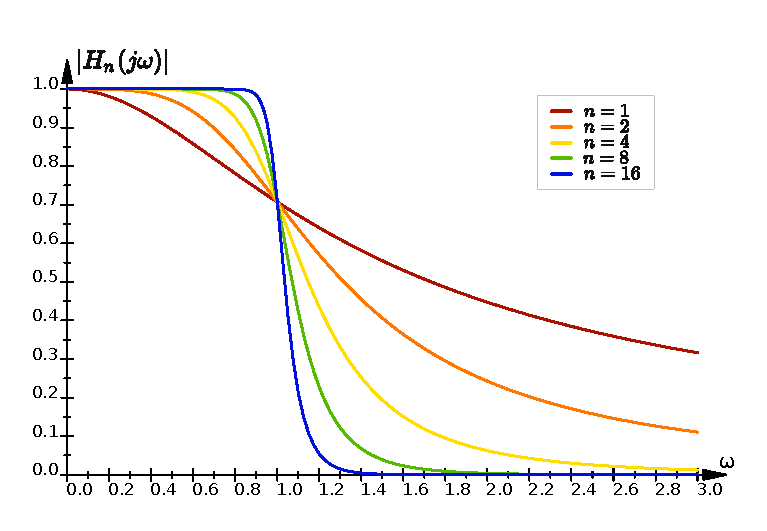
\includegraphics[width=0.9\linewidth]{./FIG/butterworth .pdf}
    \caption{Frequency response off Butterworth filter for various order}
\end{figure}


%%%Chebyshev Filter
\subsection{Chebyshev Filter}
Chebyshev Filter is signal processing filter designed in such a way that transition band has steeper frequency response than Butterworth filter.There are two types of Chebyshev filters. Type I (Chebyshev) has ripple only in Passband and Type II (Inverse Chebyshev) has ripple only in Stopband. For Chebyshev Filter  of order n, the frequency response is given by:

%%transfer function of chebyshev filter
\begin{equation*}
    {|T(jw)|}^2 = \frac{1}{1+{\epsilon}^{2}{C}_n^2(w)}
\end{equation*}
{where} $C_n(w)$ is the Chebyshev polynomial of order n.

\begin{equation*}
    C_n(\omega)= \begin{cases}
        \cos(n\cos^{-1}\omega),\quad\quad 0\leq\omega\leq 1 \\
        \cosh(n\cosh^{-1}\omega),\quad\quad \omega\geq 1
    \end{cases}
\end{equation*}

\begin{figure}[H]
    \centering
    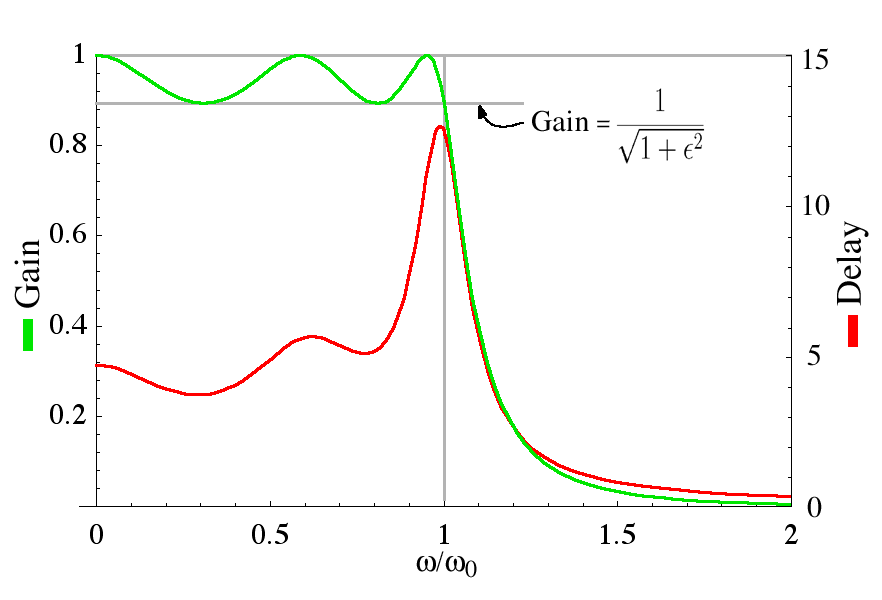
\includegraphics[width=\linewidth]{./FIG/chebyshev I.png}
    \caption{Frequency response of Chebyshev I filter}
\end{figure}

\begin{figure}[H]
    \centering
    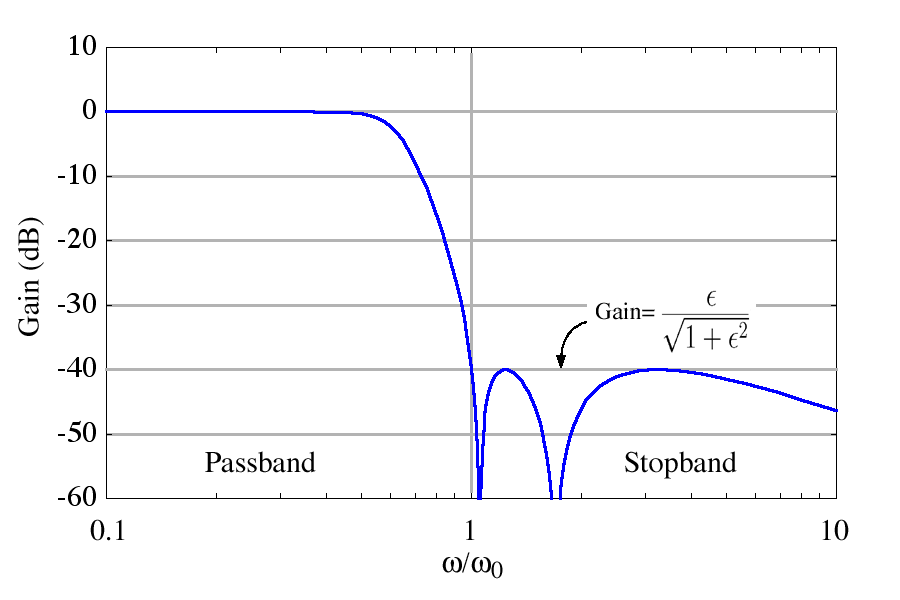
\includegraphics[width=\linewidth]{./FIG/chebyshev II.png}
    \caption{Frequency response of Chebyshev II (Inverse) filter}
\end{figure}


%%%Bessel Filter
\subsection{Bessel Filter}
Bessel Filter is signal processing filter designed to provide a constant group delay in passband thus preserving the wave shape and generally used in audio crossover system. It's frequency response is given by:

%frequency response of bessel filter
\begin{equation*}
    T_n(s)=\frac{\theta_n(0)}{\theta_n(s/w_0)}
\end{equation*}

\begin{figure}[H]
    \centering
    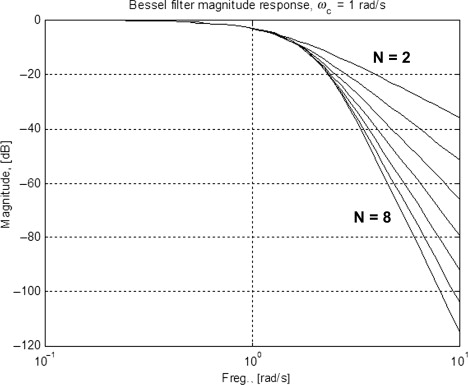
\includegraphics[width=0.5\linewidth]{./FIG/bessel.jpg}
    \caption{Frequency response of Bessel filter}
\end{figure}






%%%%%%%%%%%%%%%%%%%%%%%%%%%%%%%%%%%%%%%%%%%%%%%%%%%%%%%%%%%%%%%%%%%%

\pagebreak

%%Exercises

\section{Exercises:}

%Question 1

\begin{Q}
    {
        The circuit given in figure 1 below is a Butterworth low-pass filter having half power frequency of
        1 rad/sec. From this circuit design a lowpass filter having half power frequency of 10000 rad/sec
        and practically realizable elements. Realize the circuit, observe and plot the magnitude as well as
        phase response. Also show the highest gain in dB and half power frequency in your plot.\newline
        Observe the output in the oscilloscope when a square wave of 100 Hz is applied at input. Observe the output by increasing frequency upto 5 KHz. Comment on the result.\newline
        Typically note down the output when the square wave around 1.6 KHz is applied at input.
    }
\end{Q}


\TheCkt{Third order Butterworth Filter at half power frequency ($\omega_0$ = 1 rad/sec) }{bfilter}{\Res{1}}{\Ind{1}}{\Cap{2}}{\Ind{1}}{\Res{1}}

Given,

Half power frequency of normalized filter ($\omega_0$) = 1 rad/sec

Required half power frequency ($\omega$)= 10000 rad/sec


\begin{equation*}
    k_f= \frac{(\omega)}{(\omega_0)} = \frac{10000}{1} = 10000
\end{equation*}

To make filter practically realizable we consider Impedance scaling $K_m$ be 500

\begin{align*}
    R_{new}         & =K_m.R_{old}=500 *1=  500 \Omega                                \\
    \rightarrow R_1 & =R_2=500 \Omega                                                 \\\\
    L_{new}         & =\frac{K_m}{K_f}L_{old}=\frac{500}{10000}*1=\SI {0.05} {\henry} \\
    \rightarrow L_1 & =L_2=\SI {0.05} {\henry}=\SI {50} {\milli\henry}                \\\\
    C_{new}         & =\frac{1}{K_m.K_f}C_{old}=\frac{1}{500*10000}*2=4*10^{-7} F     \\
    \rightarrow C   & =4*10^{-7}F=\SI{0.4}{\micro \farad}                             \\
\end{align*}

\TheCkt{Butterworth Filter at half power frequency ($\omega_0$ = 10000 rad/sec) }{bfilter1}{\Res{500}}{\Indm{50}}{\Capu{0.4}}{\Indm{50}}{\Res{500}}


\Porcirobs{0.85}{a}{-6.02}{1.589}% Proteus Circuit observation Figure + table  aaaaa

No ripple is seen in Passband and transtion is gradual till stopband.



\obsh{a}
\obss{a}
\obst{a}
\obsf{a}

In above observation , in 100 Hz spikes is seen near the edges . As the frequency increases and reached 1.6kHz sine wave is seen in the middle.From 3.2 khz to 5.0 khz , the output is  getting smother.

%Question 2

\begin{Q}
    {
        The circuit given in figure 2 below is a low-pass Chebyshev filter having passband frequency of 1
        rad/sec and attenuation of 1dB. From this circuit design a lowpass filter having passband
        frequency of 10000 rad/sec and practically realizable elements. Realize the circuit, observe and
        plot the magnitude as well as phase response. Also show the highest gain in dB and half power
        frequency in your plot. Note down the ripple within the entire passband.\newline
        Observe the output in oscilloscope when square wave of 100 Hz is applied at input. Observe the
        output by increasing frequency upto 5 KHz. Comment on the result.\newline
        Typically note down the output when square wave around 1.6 KHz is applied at input.
    }
\end{Q}


\TheCkt{Chebyshev having passband frequency of 1 rad/sec and 1 dB ripple}{Cfilter}{\Res{1}}{\Ind{2.0236}}{\Cap{0.9941}}{\Ind{2.0236}}{\Res{1}}

Given,

Half power frequency of normalized filter ($\omega_0$) = 1 rad/sec

Required half power frequency ($\omega$)= 10000 rad/sec


\begin{equation*}
    k_f= \frac{(\omega)}{(\omega_0)} = \frac{10000}{1} = 10000
\end{equation*}

To make filter practically realizable we consider Impedance scaling $K_m$ be 500

\begin{align*}
    R_{new}         & =K_m.R_{old}=500 *1=  500 \Omega                                        \\
    \rightarrow R_1 & =R_2=500 \Omega                                                         \\\\
    L_{new}         & =\frac{K_m}{K_f}L_{old}=\frac{500}{10000}*2.0236=\SI {0.10118} {\henry} \\
    \rightarrow L_1 & =L_2=\SI {0.10118} {\henry}=\SI {101.18} {\milli\henry}                 \\\\
    C_{new}         & =\frac{1}{K_m.K_f}C_{old}=\frac{1}{500*10000}*0.9941=1.9882*10^{-7} F   \\
    \rightarrow C   & =1.9882*10^{-7} F=\SI{0.19882}{\micro \farad}                           \\
\end{align*}

\TheCkt{Chebyshev having passband frequency of 1000 rad/sec and 1 dB ripple }{cfilter1}{\Res{500}}{\Indm{101.18}}{\Capu{0.19882}}{\Indm{101.18}}{\Res{500}}

\Porcirobs{0.85}{b}{-6.02}{1.718}% Proteus Circuit observation Figure + table  bbbbbbb


Lowest ripple = -7.02 dB thus ripple in the passband = 1 dB

\obsh{b}
\obss{b}
\obst{b}
\obsf{b}

In above observation , in 100 Hz spikes is seen near the edges . As the frequency increases and reached 1.6kHz sine wave is seen in the middle.From 3.2 khz to 5.0 khz , the output is  getting smother.

%Queston 3
\begin{Q}
    {
        Let us modify the elements as shown in figure 3 below to have the Chebyshev lowpass filter with
        3 dB ripple. From this circuit design a lowpass filter having passband frequency of 10000 rad/sec
        and practically realizable elements. Realize the circuit, observe and plot the magnitude as well as
        phase response. Also show the highest gain in dB and half power frequency in your plot. Note down the ripple within the entire passband. Compare the response with that of problem B.
    }
\end{Q}


\TheCkt{Chebyshev having passband frequency of 1 rad/sec and 3dB ripple}{Cfilter2}{\Res{1}}{\Ind{3.3487}}{\Cap{0.7117}}{\Ind{3.3487}}{\Res{1}}

Given,

Half power frequency of normalized filter ($\omega_0$) = 1 rad/sec

Required half power frequency ($\omega$)= 10000 rad/sec


\begin{equation*}
    k_f= \frac{(\omega)}{(\omega_0)} = \frac{10000}{1} = 10000
\end{equation*}

To make filter practically realizable we consider Impedance scaling $K_m$ be 500

\begin{align*}
    R_{new}         & =K_m.R_{old}=500 *1= 500 \Omega                                          \\
    \rightarrow R_1 & =R_2=500 \Omega                                                          \\\\
    L_{new}         & =\frac{K_m}{K_f}L_{old}=\frac{500}{10000}*3.3487=\SI {0.167435} {\henry} \\
    \rightarrow L_1 & =L_2=\SI {0.167435} {\henry}=\SI {167.435} {\milli\henry}                \\\\
    C_{new}         & =\frac{1}{K_m.K_f}C_{old}=\frac{1}{500*10000}*0.7117=1.4234*10^{-7} F    \\
    \rightarrow C   & =1.4234*10^{-7} F=\SI{0.14234}{\micro \farad}                            \\
\end{align*}


\TheCkt{Chebyshev having passband frequency of 1000 rad/sec and 3 dB ripple }{cfilter1}{\Res{500}}{\Indm{167.435}}{\Capu{0.14234}}{\Indm{167.435}}{\Res{500}}

\Porcirobs{0.85}{c}{-6.02}{1.592}% Proteus Circuit observation Figure + table  ccccccc

Lowest ripple= -9.02 dB thus ripple in pass band is 3 dB.

Compared to Problem 2 sharper transition is seen in Problem 3.


%Question 4
\begin{Q}
    {
        The circuit given in figure 4 below is a low-pass Bessel filter with normalized frequency. From
        this circuit design a lowpass filter for the frequency of 10000 rad/sec. All the elements of your
        final design should be practically realizable. Realize the circuit, observe and plot the magnitude as
        well as phase response. Also show the highest gain in dB and half power frequency in your plot.\newline
        Observe the output in oscilloscope when square wave of 100 Hz is applied at input. Observe the
        output by increasing frequency upto 5 KHz. Comment on the result.\newline
        Typically note down the output when the square wave around 1.6 KHz is applied at input.
    }
\end{Q}


\TheCkt{Bessel filter at normalized frequency of 1 rad/sec}{Bfilter}{\Res{1}}{\Ind{0.337421}}{\Cap{0.970512}}{\Ind{2.203411}}{\Res{1}}

Given,

Half power frequency of normalized filter ($\omega_0$) = 1 rad/sec

Required half power frequency ($\omega$)= 10000 rad/sec


\begin{equation*}
    k_f= \frac{(\omega)}{(\omega_0)} = \frac{10000}{1} = 10000
\end{equation*}

To make filter practically realizable we consider Impedance scaling $K_m$ be 500

\begin{align*}
    R_{new}         & =K_m.R_{old}=500 *1= 500 \Omega                                                      \\
    \rightarrow R_1 & =R_2=500 \Omega                                                                      \\\\
    L_{new}         & =\frac{K_m}{K_f}L_{old}                                                              \\
    \rightarrow L_1 & =\frac{500}{10000}*0.337421=\SI {0.01687105} {\henry}=\SI {16.87105} {\milli\henry}  \\
    \rightarrow L_2 & =\frac{500}{10000}*2.203411=\SI {0.11017055} {\henry}=\SI {110.17055} {\milli\henry} \\\\
    C_{new}         & =\frac{1}{K_m.K_f}C_{old}=\frac{1}{500*10000}*0.970512=1.941024*10^{-7} F            \\
    \rightarrow C   & =1.941024*10^{-7} F=\SI{0.1941024}{\micro \farad}                                    \\
\end{align*}


\TheCkt{Bessel filter at normalized frequency of 1000 rad/sec }{bfilter1}{\Res{500}}{\Indm{16.87105}}{\Capu{0.1941024}}{\Indm{110.17055}}{\Res{500}}

\Porcirobs{0.85}{d}{-6.02}{1.589}% Proteus Circuit observation Figure + table  dddddd

\obsh{d}
\obss{d}
\obst{d}
\obsf{d}

In above observation , in 100 Hz spikes is seen near the edges . As the frequency increases and reached 1.6kHz sine wave is seen in the middle.From 3.2 khz to 5.0 khz , the output is  getting smother.

%Conclusion

\section{Discussion \& Conclusion}
In this Lab  we did comparison of magnitude \& phase response different Filter Networks. We used  Proteus  design suite to design and plot frequency response for the circuit. We studied and design practically realizable Butterworth, Chebyshev and bessel filters.

\end {document}